% !TEX root = ../../my-thesis.tex
%
\graphicspath{{./content/introduction/figures/}}

\chapter{Introduction}

\cleanchapterquote{Nature loves to hide.}{Heraclitus (c. 6th-5th century BCE)}{}


\label{chap:intro}

% \cleanchapterquote{Le bout du monde et le fond du jardin contiennent la même quantité de merveilles.}{Christian Bobin}{(French poet)}

% TODO : investigate the difference between frequency dependence, density dependence, and the likes , cf \citep{Lion2022}
\section{Context}

\subsection{Biological and economic systems as complex adaptive systems}
%% definition of complex adaptive system
What are the similarities between the dynamics of biological and economic systems? 
% 
Think of a biological system as a community of interacting biological organisms \citep{chapin2002principles}, and think of an economic system as a community of interacting economic agents \citep{Dopfer2007}.
% 
The dynamics of a biological system depends on fluxes of matter and energy between organisms, and the dynamics of an economic system depends on fluxes of capital between economic agents.
% 
\textit{A priori}, the underlying processes strongly differ, because the behavior of economic agents is motivated by rationality, where economic agents maximize utility \citep{10.1093/cje/bet027}. 
% 
Nonetheless, economic agents are faced with uncertainty \citep{Foster2012} and their rationality is bounded \citep{Veblen1898,nelson1985evolutionary}. As a result, economic agents adopt a variety of behavioral rules (e.g. technological, organizational, institutional, see \cite{Foster2012}) through trial-and-errors, which are subject to natural selection through competition processes \citep{schumpeter2017theory}.
% 
In this perspective, both biological and economic systems are complex adaptive systems \citep{Levin2002}, composed of heterogeneous entities that interact in nonlinear ways and experience evolutionary processes. 
% 
% Interaction and evolutionnary processes take many different forms and operate at different organizational level \citep{Levin1998} (see \cref{fig:organisational_levels}).
% 
The processes of interaction and evolution involved take many forms and operate at different organizational level \citep{Levin1998}, from genes to ecosystems, and from organizational routines to economies, with feedback mechanisms between the organizational levels (see \cref{fig:organisational_levels}).
% 
Interestingly, the stochasticity of the processes involved, and their couplings, do not necessarily lead to unpredictable structures and dynamics, but rather induce organized structural properties and invariant patterns \citep{Olff2009,mitchell2009complexity}. 
% 
In biological systems, invariant patterns include patterns of species richness, where for instance montane regions are often associated with a disproportionately high number of species \citep{Rahbek2019}. In economic systems, invariant patterns include the bimodal shape of the distribution of international income, where some countries have systematically developed much more rapidly than others \citep{acemoglu2001colonial}. 
% 
A common direction on the research agenda in biology and economics is to understand general organizational principles, i.e.  to underpin the fundamental processes and feedbacks that generate invariant patterns \citep{Levin2002,Olff2009,Veldhuis2018}.
% 
In biological systems, the fundamental processes resulting in patterns of species richness are identified \citep{Rahbek2019a,Rangel2018,Hagen2022}, and the current challenge is to underpin the mechanisms resulting from their couplings \citep{Hagen2022}.
% 
In economic systems, we still do not exactly understand the fundamental processes at stake. 
% 
% Example : biology
% For instance, in biological systems, mountane regions are often associated with a disproportionately high number of species \citep{Rahbek2019}, and the proposed hypotheses involve a hierarchy of processes acting at different organization scale including populations, species and assemblages \citep{Rangel2018,Rahbek2019a}.
% % 
% %% Example: economics
% Similarly, in economic systems, the distribution of international incomes is bimodal \citep{acemoglu2001colonial}, and economic processes at the national and subnational levels, and their interplay, have been proposed as determining factors \citep{Hidalgo2021,C.A.HidalgoB.Klinger}.
% 
%% limitations of the current understanding
% 
% conclusion
% Although being observed in distinct systems with singular characteristics, these emergent patterns may have been shaped by analogous forces.

%% Figure parallels
\begin{figure}[ht]
    \centering
    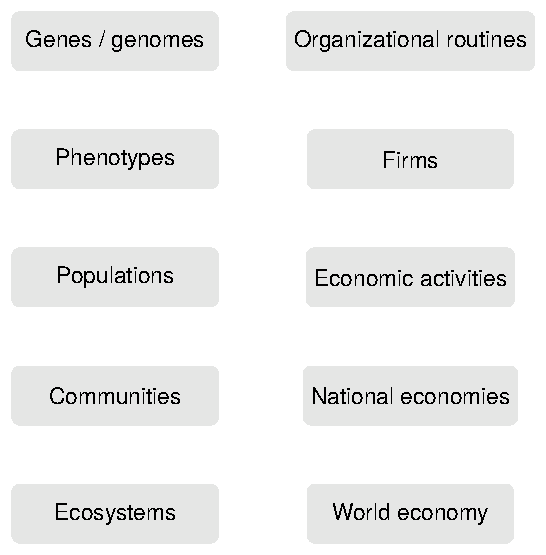
\includegraphics{organizational_complexity.pdf}
\caption{Graphical representation of organizational levels and their couplings in biological and economic systems. An arrow indicates that the organizational level at its tail can influence the organizational level at its head. Left diagram is inspired from \cite{Hendry+2016}.}
\label{fig:organisational_levels}
\end{figure}

%% Figure micro / macro properties




\subsection{Ecological and evolutionary processes drive the dynamics of biological systems}
% 
% History of the understanding of forces in ecology and evolution
% The challenge is to bridge the microscopic processes developing at a lower organizational level to deduce the long-term dynamics of these macroscopic features.
% % 
% The difficulty is to comprehend the coupling between the processes of interaction and evolution \citep{Strogatz2001a}. The former correspond to ecological processes, and involve fluxes of energy and matter across space and time, encompassing the processes of interaction between organisms (biotic interactions) and between organisms and their environment (abiotic interactions), and dispersal processes (movement of individual across space) \citep{Vellend2010a}. This term may also designate fluxes of information and capital between economic agents \citep{}.
%
% Biological systems are ruled by processes that have traditionally been grouped into two distinct classes, namely ecological and evolutionary processes \citep{Pelletier2009}.
% 
In biological systems, interaction processes are more commonly designated as ecological processes, and encompass the processes of interaction between organisms (biotic interactions) and between organisms and their environment (abiotic interactions), as well as dispersal processes (movement of individual across space) (\cite{Vellend2010a}, see \cref{fig:eco_evo} for a graphical representation).
% 
Evolutionary processes designate those processes responsible for the change of heritable characteristics (DNA, genes, phenotypes) over successive generations (\citep{Hall2013}, \cref{fig:eco_evo}).
% 
The coupling between ecological and evolutionary processes is acknowledged since the very birth of the theory of evolution. 
% 
During his voyage on the Beagle, Darwin documented a link between the different ecological opportunities across the Galápagos Islands and the different beak shapes in the finches he found on each island \citep{darwin2004origin}.
% 
He reasoned that the variations in ecological opportunities lead to a differential in survival for certain phenotypes, which over time resulted in the evolution of different beak shapes.
% 
Since then, we know that ecological processes interact with evolutionary processes, and they together shape the long term dynamics of biological systems \citep{Rahbek2019a,Rangel2018,Hagen2022}.
% 
Empirical studies have now demonstrated that evolution can be rapid and occur on similar time scales as ecology \citep{Hairston2005, Pelletier2009} and have quantifiable effects on ecological dynamics \citep{Ezard2009}, leading to feedbacks between ecological and evolutionary processes, so-called eco-evolutionary feedbacks \citep{Pelletier2009,Schoener2011,Govaert2019}. 
% 
% Example of eco-evolutionary dynamics
Eco-evolutionary feedbacks involve situations where an ecological process (e.g., replication, competition, dispersal) influences an evolutionary process (e.g. phenotypic change), which then feeds back to an ecological process, or vice versa (\cite{Govaert2019}, \cref{fig:eco_evo}). Examples are feedbacks between population dynamics (replication and competition) and phenotypic change, which can lead to evolutionary branching through the effect of competition \citep{Dieckmann1999}.
% 
In spatially structured populations, another classical example of eco-evolutionary feedbacks is the mechanism of local adaptation \citep{Savolainen2007}, where feedbacks between population dynamics, dispersal and trait evolution can facilitate or prevent populations to adapt to local environmental conditions \citep{Meszena1997,Doebeli2003}.
% 
Importantly, the eco-evolutionary feedbacks involved in adaptation mechanisms are expected to affect the dynamics of ecosystems in the coming decades \citep{Norberg2012,Urban2016}, because of the expected rapid changes in environmental conditions due to anthropogenic pressure and climate change \citep{Ellis2011,Midgley2019}.
% 
Nevertheless, our understanding of eco-evolutionary feedbacks in realistic biological scenarios is limited \citep{Lion2022}.
% Eco-evolutionary feedbacks are also involved in adaptation mechanisms \citep{Doebeli1999}, where species disperse and phenotypic variations allow to adapt to local environments \citep{XXX}.
% TODO: mention density dependence
% Empirically, \citep{XXX} shows that in the population of XX, XX happened.
% 
% In order to mitigate the consequences of human development, it is of utmost urgency to better understand eco-evolutionary feedbacks \citep{Norberg2012}, and develop mechanistic models embedding this knowledge \citep{Urban2016}. This will in turn provide more reliable forecasts of ecosystem states \citep{Clark2001}, to help designing adequate management of ecosystem services \citep{Urban2016}.
% 
% Advancing our understanding  in realistic biological scenarios \citep{Lion2022}. 
% In particular, the answer to how species will adapt to increasing temperatures is uncertain due to our lack of understanding of eco-evolutionary feedbacks \citep{Norberg2012}. 
% 
% They are critically involved in adaptation mechanisms, which calls for 
%% Conclusion
% While eco-evolutionary feedbacks may greatly influence the mechanisms driving the dynamics of ecosystems \citep{Urban2016}, our quantitative understanding of their modality is limited \citep{Lion2022}. 
% 
% Beyond raising questions of sheer scientific interest, gaining such an understanding is a pressing need to mitigate the effect of global change.

\begin{figure}[ht]
    \centering
    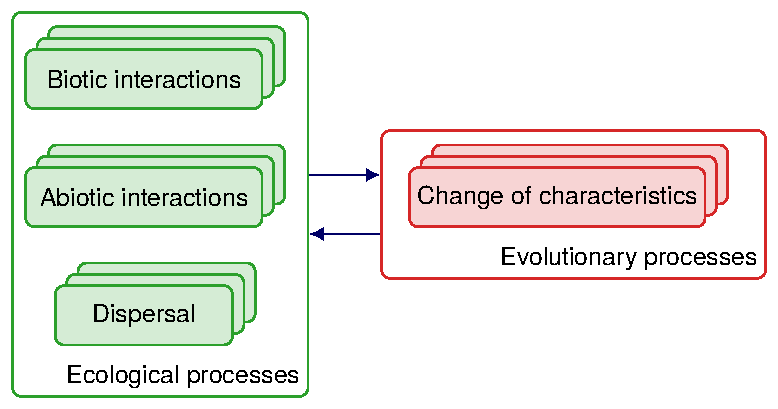
\includegraphics{eco_evo.pdf}
\caption{Graphical representation of the eco-evolutionary processes determining eco-evolutionary dynamics in biological. By extension, I use this terminology to designate interaction and evolutionary processes in economic systems.}
\label{fig:eco_evo}
\end{figure}

\subsection{Drivers of economic change}
In economic systems, the fundamental processes determining economic change are controversial \citep{Dopfer2007,Nelson2014,Hodgson2019}. 
%  This idiosyncrasy has been traditionally explained by geographic and institutional arguments \citep{C.A.HidalgoB.Klinger}. 
%% Mainstream econoomics vs evolutionary economics
To explain economic development, the neoclassical theory \citep{10.1093/cje/bet027} assumes that economic systems are in equilibrium, in the sense that the demand and supply of goods and services are balanced on all relevant markets. 
% TODO: Marks comments : transition from countries to firms is not quite clear to me here
Firms are rational in maximizing profits by adapting to demand and supply, and the observed economic change is driven by exogenous forces, such as technological change \citep{Romer1986}. Evolutionary economics, promoted by the seminal work of \cite{Nelson2014}, criticizes this view and seeks to explain economic change by focusing on endogenous forces. 
% 
%% Foundations of evolutionary economics
Evolutionary economics suggests that interactions between economic agents, firms and economic activities, and evolutionary processes acting upon them, are major processes contributing to economic change \citep{Hodgson2019}.
% 
These interactions may consist in facilitation processes through supply chains \citep{Ozman2009,Saavedra2009a,VanDerPanne2004} or competition within markets \citep{Wernerfelt1989}. What determine these interactions, and firm and economic activities' behavior in general, are organizational routines (\cref{fig:organisational_levels}), which spread across space and adapt \citep{Cordes2006}, affecting economic development at the local, regional, national, and international scale.
%
%% biology as a way to understand economic dynamics
% Because such processes are analogous to the processes shaping the dynamics of biological populations and ecosystems, notorious economists such as Veblen \citep{Veblen1898} or Arrow \citep{doi:10.1126/science.267.5204.1617.g} have proposed that the appropriate paradigm to understand economic change should be evolutionary biology.
% 
% TODO: The processes of interaction and dispersal are analogous to ecological processes operating in biological systems \citep{XXX}, in that they also involve fluxes (of matter, information, and capital) between economic agents. By extension, we use eco-evolutionary processes and dynamics both in biological and economic systems.
% 
Because these proposed processes are analogous to eco-evolutionary processes driving the dynamics of biological systems (which motivates the use of this terminology for designating economic processes in the following), a number of modelling approaches have borrowed concepts and methods from biology, aiming at underpinning the fundamental processes underlying invariant patterns in economic systems \citep{Tacchella2018,Saavedra2009a,Scholl2020,Zhang2018,Modis1997,Saavedra2014,Farmer1999,Michalakelis2011,Marasco2016,Gatabazi2019,Cauwels56,Applegate2021,Suweis2015}. 
% 
For instance, \cite{Saavedra2009a} has successfully used a model of mutualistic interaction to explain structural patterns in industrial cooperation.
% 
Also, \cite{Scholl2020} uses the concepts of food webs and density dependence to explain market malfunctions and excess volatility in financial markets.
% 
However, those studies did not seek to understand how eco-evolutionary processes may affect economic development at the national scale.
% 
Biologically inspired eco-evolutionary models may help to disentangle the effect of eco-evolutionary processes on the dynamics of national economic systems, and could explain differences in economic development across countries.

\section{Modeling eco-evolutionary dynamics}

\subsection{Forward modelling of eco-evolutionary processes}
The complex interplay between ecological and evolutionary processes can hardly be studied with experimental approaches (\cite{Pontarp2019,Hagen2022}, but see \cite{Becks2012} for an experimental study with rotifer-alga microcosms). 
% TODO: cite \citep{May2004}
As such, a deductive approach, relying on forward modelling, has traditionally been put forward to underpin the mechanisms underlying invariant patterns in biological systems \citep{Brummitt2020}. Along this approach, hypotheses about causal processes are embedded in a model, whose simulation (integration) generates emergent (non-anticipated) properties (see \cref{fig:forward_inverse_modelling}). Emergent properties may be seen as predictions from the consideration of the processes considered \citep{May2004}, and the role of the modeler is to underpin the underlying mechanisms, i.e. to disentangle how the interplay between the processes generate the observed behavior. 
% 
% The resulting qualitative dynamics and/or quantitative predictions are validated against common intuition and empirical data, and further refined to elaborate a theory \citep{Sayama,Brummitt2020,Schmidt2009}.
% 
%% early mathematical models
In the early 1930s to 1940s, by formulating tractable mathematical models implementing the processes of reproduction, dispersal and mutations, the work of Fisher, Wright and Haldane has greatly contributed to the modern synthesis of evolutionary biology \citep{huxley1942evolution}, generally accepted as the basis of our current understanding of evolutionary dynamics. 
% 
% The mechanistic models commonly take the form of differential equations (DE), and express how the processes under investigation affect the rate of change of the population characteristics, such as the proportion of a given allele. 
% 
Yet in order to obtain tractable mathematical model, Fisher, Wright and Haldane have neglected eco-evolutionary feedbacks \citep{Govaert2019}. In particular, ecological processes have been strongly simplified, and the effect of evolutionary processes on population dynamics has been neglected \citep{Lion2022}.

%% computers
With the increase in computational capacity, novel modelling approaches relying on individual based models (IBMs) have appeared \citep{deangelis2005individual}. These models require less simplifying assumptions than traditional mathematical models \citep{deangelis2005individual}, and can unveil more realistic mechanisms by allowing to capture processes acting at the individual level. However, the lack of analytical tractability of IBMs is a shortcoming, because it challenges the ability of the modeler to underpin general principles from the simulations \citep{Lion2016,May2004}.
% 
%% computers and analytical framework
The recent development of mathematical techniques, such as moment closure approximations \citep{law1999moment,Gandhi2000,Nordbotten2020,Lion2016}, adaptive dynamics theory \citep{Metz1995}, and probability theory \citep{Champagnat2006}, are generating novel pathways by filling the gap between IBMs and mathematical models. 
% 
% They allow to derive analytical expressions for the population macroscopic properties (e.g., population size and trait variance) from individual-based assumptions. 
% 
Analogous to renormalization group analysis developed in quantum and statistical physics \citep{Sayama}, they form a toolbox to rigorously derive how emergent properties are influenced by processes operating at different organizational levels. As such, these mathematical techniques allow an analytical underpinning to IBM simulations, and can generate a general understanding of the key mechanisms at stake \citep{Lion2016}.

%% examples of the combination of computer models and analytical tools
The combination of numerical simulations and, e.g., adaptive dynamics theory, has successfully shed new lights on the emergence of evolutionary branching under feedbacks between population dynamics and phenotypic change \citep{Dieckmann1999,Doebeli2003}.
%
An other example is the work of \cite{Meszena1997,Debarre2013, Mirrahimi2020}, that has provided new insights on the effect of habitat heterogeneity on local adaptation. 
% 
However, our current understanding of eco-evolutionary feedbacks neglects specificities of real biological populations that may significantly alter the resulting mechanisms, such as the structuration of populations over complex spatial structures \citep{Nowak2001a} and highly dimensional phenotypic space \citep{Doebeli2010}.

% 
% For instance, the spatial scenario investigated in \citep{Gandon, Mirrahimi2016} merely involves two habitats, and it is unclear how their results would apply to more complex landscapes, such as mountains \citep{Rahbek2019}.
% 
The consideration of such factors is important to advance our understanding, but raises challenging methodological issues. 
% 
In particular, adding complexity in eco-evolutionary models may hinder the fundament mechanisms underlying the emergence of a pattern.
% 
Also, the consideration of multiple traits leads to an increase in the dimensionality of the model, which in turn leads to an exponential increase in the computational cost associated to the numerical simulations \citep{Bellman1957}.
% 
In order to better understand eco-evolutionary dynamics, we need to investigate more realistic scenarios, which in turn require methodological developments, in order to cope with the extra complexity and computational cost.
% TODO: Marc;s comments: I like the last sentence that connects back to th eco-evolutionary modelling. It's a good introduction to the modelling approaches and well writen, but somehow I find it no so well connected to the problem. Maybe it's just because I don't fully understand :-)
% 
% This understanding uses matrices or networks to create representations of complex systems that do not ignore the identity of the elements involved or their interactions. These ideas, which are now prevalent in fields such as machine learning and physics, have begun to make their way into economics under the umbrella of economic complexity

\begin{figure}[t]
    \centering
    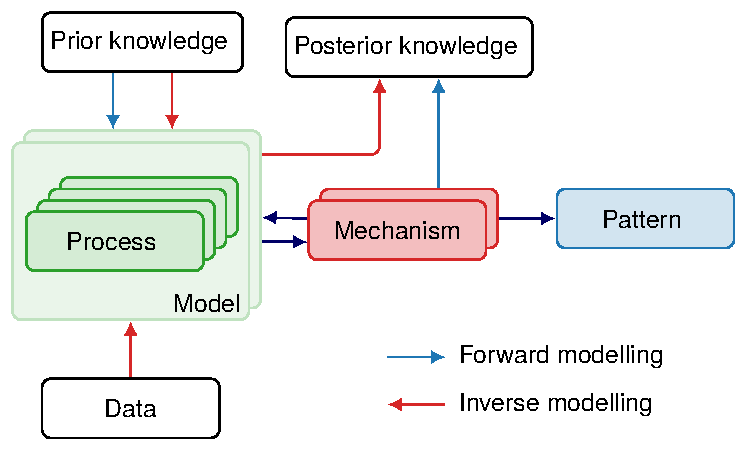
\includegraphics{forward_inverse_modelling.pdf}
    \caption{\textbf{Forward and inverse modelling approaches for the understanding of complex adaptive systems}. A forward modelling approach consists in deriving a model, embedding a set of processes inspired from prior knowledge. The objective is to understand how the interplay between the processes considered transforms in (feedback) mechanisms that are associated with an invariant pattern. An inverse modelling approach integrates empirical observation within the modelling process. Posterior knowledge on the empirical system is obtained whether form the interpretation of the estimated parameter values, or through model selection.
    % Similarly to forward modelling, mechanisms resulting from the interplay between the processes and involved in invariant patterns may be investigated.
    }
    \label{fig:forward_inverse_modelling}
\end{figure}

\subsection{Inverse modelling}
%% inverse modelling
Another approach to underpin processes and mechanisms in biological systems consists in inverse modelling, where empirical data is used to constrain the model (\cite{Clermont2015}, see \cref{fig:forward_inverse_modelling} for a graphical illustration).
% 
% While in forward modelling, observation data is uniquely considered at the end of the modelling cycle - when comparing predicted and empirical patterns to refine prior knowledge on the system investigated -, inverse modelling integrates empirical data right at the start the modelling cycle to characterise the processes involved \xxx .
% 
% Diametrically opposed to forward modelling, inverse modelling consists in using observation data to infer causal processes \citep{Peng2011}. Inverse modelling has recently seen an increased attention, thanks to the increased computational power and availability of datasets \citep{Csillery2010}.
% 
%% Parameter estimation
% TODO: may be to modify, to say that inverse modelling consists in parameter estimation, which is the first step of model selection
Inverse modelling can take the form of parameter estimation \citep{Schartau2017} or model selection \citep{Johnson2004}, both involving the use of inference methods to estimate, respectively, the most probable model parameter value, or the most probable model among candidates, given empirical data.
% 
% involves the use of inference methods to estimate the most probable model parameter value given the data \citep{Schartau2017}. They can also be used to test the support of competing hypotheses, embedded in alternative models, where 
% 
% such as bayesian or maximum likelihood inference methods . 
% 
% Those methods proceed by defining a distance between the model simulation and the observation data, which relates to the probability of the parameters given the model and the data \citep{Schartau2017}. The most likely parameters are associated with the minimum distance, obtained using ad-hoc algorithms.
% 
In parameter estimation, provided that they are inferred together with uncertainties, parameters can be interpreted to better understand the strengths and effects of the processes considered \citep{Pontarp2019}. For instance, \cite{Higgins2010,Curtsdotter2019} infer the parameters of population dynamic models to understand the processes involved in ecosystem functions.
%
In model selection, candidate models embedding competing hypotheses about causal processes are derived, and the relative support of each model given the data is computed to discriminate between the hypotheses \citep{Johnson2004}. For instance, using inverse modelling and alternative eco-evolutionary models, \citep{Skeels2022} shows that temperature-dependent evolutionary speed most likely explains variations in biodiversity patterns, among alternative evolutionary speed hypotheses.

The computation of the most probable model parameter values, or the computation of the different model supports, critically involves inference methods. %Inference methods proceed by characterizing the global, or minimum, distance between the model simulation and the observation data \xxx, which relates to the probability of the data given the model and the parameter values \citep{Schartau2017}. %In parameter estimation, the most likely parameters are associated with the minimum distance to the data \xxx, and in model selection, the most likely models are associated with the minimum of the minimum model distance \xxx.
% 
Inference methods commonly demand many forward integration of the model, resulting in a computational cost that can be prohibitively expensive \citep{Schneider2017}.
% 
The number of forward integration required may dramatically increase with the number of model parameters \citep{Csillery2010}, and the number of model parameters, together with the model nonlinearities, can eventually lead to false estimates of the most probable model parameter values \citep{Gabor2015}.
% 
% The success of inference methods is further limited by the complexity of the models involved , where the number of model parameters, the computational cost associated to the model integration, and the model nonlinearity prevent to correctly approximate the distance.
% 
Consequently, inverse modelling methods have mostly been used with simple evolutionary models \citep{Csillery2010}. 
% 
Eco-evolutionary models are dependent on numerous parameters \citep{Boyd2012}, are strongly nonlinear \citep{Hastings1993,Huisman1999,Beninca2008}, and their integration is computationally expensive \citep{Fisher2018}, challenging the use of inverse modelling to underpin eco-evolutionary processes. 
% 
Advances in the field of artificial intelligence could circumvent these issues, allowing to advance our knowledge of eco-evolutionary dynamics in empirical systems.  
% 
% Inference methods involve numerical methods to recover the model distance to the data \xxx, which success is dependent on the model formulation and its dynamical properties \xxx.
% 
% The parameter estimation problem consists in finding the maximum probability of the model given the observation data, inference methods can also be used to discriminate between candidate mechanisms embedded in alternative models \citep{Burnham2002,Johnson2004}. For instance, \citep{Skeels2022} shows that temperature-dependent evolutionary speed is the most likely mechanism to explain variations in biodiversity patterns, using inference methods to discriminate between alternative dynamic models embedding different hypotheses.
% 
% For instance, \citep{Higgins2010,Curtsdotter2019} infers and analyse the parameters of population dynamic models to understand processes involved in ecosystem functions.
% 
% Thus far, the use of inverse modelling for understanding eco-evolutionary dynamics has been limited because of a number of issues, including the high computational cost of the forward integration of eco-evolutionary models \citep{Fisher2018}, the large number of parameters involved \citep{Boyd2012}, and their strong nonlinearities 

% TODO: Victor, you stopped here on the 15th of September.
\subsection{Artificial intelligence to leverage forward and inverse modelling}
\label{subsec:AI}
In the recent years, the field of artificial intelligence (AI) has made enormous progresses in computer vision \citep{voulodimos2018deep} and natural language processing \citep{young2018recent}. At the backbone of this success are key computational techniques that could leverage the forward and inverse modelling of eco-evolutionary dynamics.
% 
% AI uses observation data to learn abstraction of mechanisms and make prediction about the world, 
% 
%% AI and neural networks
% 
% Neural networks are universal approximators \citep{XXX}, i.e. parametric functions that can theoretical approximate any high dimensional function, such as the function that allows us to differentiate a cat from a dog.
% 
% Neural networks are computational models with very good properties to interpolate data \citep{xxx}, and have been used, for instance, to build species distribution models from occurrence datasets \citep{Deneu2021}.
% 
Advances in computer vision and natural language processing rely on deep learning methods, that allow neural networks to learn abstract representation of mechanisms from large datasets \citep{LeCun2015}.
% 
These abstractions can hardly be interpreted to generate scientific theories \citep{Karpatne2017}, and their prediction ability is limited by the information contained in the training datasets. As such, neural networks cannot be used \textit{per se} to gain scientific insights and extrapolate beyond observed trends \citep{Barnosky2012,Urban2016}. %Last but not least, the success of the learning process in tightly linked to the quantity of data available for training. Yet in many scientific domains -- comprising evolutionary biology and economics -- the expense, or impossibility, of conducting experiments prohibits the collection of large datasets.
% 
Nevertheless, their traditional applications and associated methods have been successfully derived in other scientific fields for this purpose \citep{Kashinath2021,Schneider2017,Yazdani2020,Rolnick2023}.
%
%% ML for forward modelling
Neural networks have been used to reduce the cost of the forward integration of climate models, learning more efficient representations of physical mechanisms \citep{Kashinath2021}.
% 
They have also been used to approximate the solution of partial differential equation (PDE) models \citep{Sirignano2018dgm,Han2018}, with the major advantage of approximating high dimensional problems at a lower computational cost than traditional methods.
% 
% Notoriously, \citep{Arnulf} has developed methods consisting in training neural networks through a correspondence between PDEs and stochastic processes. \citep{Arnulf} have mathematically proved and numerically showed that their methods can efficiently approximate very high dimensional PDEs (10 000 dimensions), which could allow to include more realism in eco-evolutionary models.
% 
% Nonetheless, PDE models for CAS critically involve non-local terms, which capture non-local interactions between microscopic agents. The extension of such techniques to non-local PDEs could leverage the forward modelling of biological and economic systems.
%
%% ML for inverse modelling
% Neural networks have also been employed to leverage inverse modelling techniques.
% 
Underlying the training of neural network is the technique of backpropgation \citep{LeCun2015}. This technique can be generalized to train any scientific model against data \citep{Rackauckas2020}, with the potential to leverage inverse modelling techniques \citep{Frank2022}. %With the ability to handle computational models characterised by a very large number of parameters, AD, together with the development of other training techniques \citep{XXX}, have the potential to leverage inverse modelling \citep{Rackauckas2020}.
% 
% For instance, automatic differentiation has allowed symbolic regression, automatically generating symbolic equations for nonlinear coupled dynamical systems directly from time series data \citep{WOS:000247363000007}. Cons: this method is "model-free", and is rather more relevant in engineering. It generates equation from a bank of polynomials, but is not suited for testing a bunch of different models. It also handle model with simple dynamics, while real-world systems often show chaotic dynamics. Identifying only the useful analytical relations that are related to the system dynamics. still faced with the challenge of justifying and giving words to their meaning. One difficulty is that we cannot know with certainty the units of bulk constants in the law ex- pressions (for example, combinations of masses, lengths, etc. embodied in the system). Second, the equation may model something that is inherently difficult to observe directly, such as total energy. Requiring equations to maintain consistent physical units still leaves room for ambiguity. \citep{Schmidt2009} \citep{Mangan2017}.
% 
Consequently, AI techniques offer unique opportunities for advancing our understanding of eco-evolutionary dynamics.

% to be checked tomorrow (01/09)
% Recent advances in interpretable ML are enbling the generation of theories to be automated. Mathematical laws, that took many years for scientists to solve manually, have been identified in physical and biological systems.

% the abstractions that they learn from the data is inscrutable
% This learning process is allowed by using the backpropgation algorithm, to indicate how a machine should change its internal 

% The predictive ability of mechanistic models has remained poor \citep{DeAngelis2015}, due to a low pervasion of observation data in mechanistic models \citep{XXX}.

\subsection{Programming languages}
\label{subsec:Julia}
Combining AI techniques with scientific models requires a computational environment that allows to easily develop scientific models, while ensuring simulation performance, and providing composability between AI and other scientific libraries \citep{Rackauckas2020}. Unfortunately, performance and composability are features that are poorly represented in mainstream programming languages used by the scientific community, such as Python, Matlab or R.
% 
%% performance and ease of use
Those languages are naturally attractive because they are dynamically typed \citep{Bezanson2017}, allowing convenient development iterations. Nonetheless, prototypes written in Python, Matlab or R need to be rewritten in low level, compiled languages such as C, C++ or Fortran for speed and predictable mapping to hardware \citep{Perkel2019,Bezanson2017}. This conversion requires significant efforts, leading to a problem commonly designated as the "two-language problem" \citep{Bezanson2017}.
% 
In order to circumvent performance issues, most libraries in Python, Matlab or R rely on bindings with low level languages. For instance, the most used deep learning libraries in Python, TensorFlow and PyTorch, are internally written in C++ (see \cite{tensorflow,pytorch}). However, bindings with low level languages come with major negative externalities. First, they restrict the understandability of their source code to computer scientists -- prohibiting potential development contributions from the scientific community. Second, they prevent the composability of, e.g., traditional scientific computing libraries and deep learning libraries \citep{Innes2019}. This absence of composability arises because deep learning libraries must differentiate the numerical models to be trained. Yet, TensorFlow or PyTorch are only able to differentiate models written in their own internal source code \citep{Innes2019}.

%% Julia 
Julia is a recently developed programming language that addresses the issue of the two-language problem \citep{Bezanson2017,Bezanson2018}. Julia was built over a type-specializing, just-in-time compiler, which makes it easy to generate performant programs in pure Julia, while preserving the essential features of Python, Matlab or R, such as dynamic typing and automatic memory management \citep{Perkel2019}. 
% 
The source code of most Julia libraries is consequently written in pure Julia, guaranteeing understandability and composability.
% 
In particular, Julia is an automatic differentiation pervasive language \citep{Innes2019}, which allows to differentiate any model written in pure Julia without any modification. As a result, deep learning libraries can be used on any scientific model written in Julia \citep{Rackauckas2020a}.
% 
Solving the two-language problem, Julia permits scientists to prototype a program which is readily generic and performant, benefitting not only the development process but also the entire research community \citep{Bezanson2017}.
% 
% This unique feature has motivated the Climate Modelling Alliance to build an entirely new climate model in Julia, in order to obtain compatibility with ML libraries with the aim of improving predictions with data \citep{Tapio}.
% 
Overall, the composability and productivity granted by Julia makes it an ideal computational environment to accelerate research. 

\section{Thesis outline}

In summary, while it is increasingly acknowledged that feedbacks between ecological and evolutionary processes play an important role in biological systems \citep{Pelletier2009, Urban2016}, our understanding of eco-evolutationary dynamics in realistic scenarios is limited.
% 
Under increasing anthropogenic pressure, advancing this understanding is essential \citep{Urban2016} but raises challenging methodological issues.
% 
Further, while analogous processes to eco-evolutionary processes have been suggested to influence the dynamics of economic systems \citep{Hodgson2019}, we do not know their effect on economic dynamics at the scale of a country.
% 
Here, I present novel forward and inverse modelling approaches to advance our understanding of eco-evolutionary dynamics, and utilize them to shed light on the eco-evolutionary processes and feedbacks in biological and economic systems.


In \cref{chap:diff-in-graphs}, I investigate how eco-evolutionary processes, in combination with complex habitat structures, influence the phenotypic distribution of biological populations. 
I proceed using a forward modelling approach: I derive a stochastic eco-evolutionary IBM where individuals are structured over a spatial graph, and experience the fundamental processes of reproduction, competition, mutation and migration. Seeking to understand how those processes result in phenotypic differentiation at the population level, I derive analytical approximations of the IBM. Together with extensive numerical simulations, they provide insights into how the graph properties affect the population size and phenotypic differentiation. In particular, I show that three main graph properties, relating to landscape connectivity, heterogeneity in connectivity, and habitat spatial auto-correlation, shape phenotypic differentiation. These results establish mechanistic links between landscape features and the eco-evolutionary dynamics of biological populations.

In \cref{chap:mini-batching}, I develop an inverse modelling method to estimate the parameters of eco-evolutionary models and perform model selection. The method is based on a machine learning framework and involves the combination of state-of-the-art AI techniques and a novel learning strategy. The learning strategy consists in training the model against mini-batches of data with short time horizon, which I analytically show to bypass problems arising from model nonlinearities. I implement the ML framework in a new Julia library released under the name of \textbf{MiniBatchInference.jl}, and demonstrate through numerical experiments that it can efficiently and accurately estimate model parameters and provide model support from noisy, incomplete and independent time series. Altogether, the proposed ML framework is a workhorse for inverse modelling and can elucidate mechanistic pathways in biological and economic systems.

In \cref{chap:econobiology}, I quantify the effect of eco-evolutionary processes on the dynamics of economic systems. I employ the ML framework developed in \cref{chap:mini-batching} to investigate how alternative eco-evolutionary population models can explain the dynamics of economic activities in 74 of the world's richest countries, relying on 59 year of economic data. The models embed processes acting upon economic activities, including ecological interactions between them, their spatial dispersal, and their transformaton transformations. The statistical support of each model is compared to a simple logistic growth model, taken as a null model. I find strong statistical evidence for positive interactions between national economic activities, and spatial dispersal. To my knowledge, this is the first study providing quantitative evidences that eco-evolutionary processes shape the dynamics of economic systems.

In \cref{chap:nonlocalPDE}, I extend two recent methods to solve high dimensional non-local nonlinear PDEs. This class of PDEs can be used to construct generic eco-evolutionary models capturing the evolution of complex phenotypic populations, but up to now, could only be simulated in low dimensions. The first method presented relies on Picard iterations, while the second is based on deep learning and involves neural networks to approximate the PDE model output. I implement both methods in the Julia library \textbf{HighDimPDE.jl}, and evaluate their performance on high dimensional eco-evolutionary models, and on PDE models arising in physics. The methods yield good results with short run times, opening up new venues to further our understanding of eco-evolutionary dynamics.

\newpage

% remains to be understood, and is more important than ever in a rapidly changing world.

% \section{Complex adaptive systems}
% \label{sec:intro:cas}
% \begin{outline}
%     \1 A central aim in the discipline of Ecology is to determin the underlying causes of variation in the abundance and sitribution of species.
%     \1 Ecological and economic systems are complex adaptive systems (CAS): they are systems that are composed of many entities with heterogeneous characteristics, which interact and experience selection processes. Those processes act at the individual level, but are key in determining the macroscopic behaviour at the system level, a feature that make those systems unique.
%     \1 Complex interconnected systems pose a major challeng to scientific study in ecology and economics \citep{Ye2016} (and references therin).
%         \2 the common approach of reducing these systems to linearly independent components overlooks important interactions for the sake of computational tractability 
%         \2 statistical frameworks (e.g., PCA, GLM, multivariate autoregressive models), assume that caysal factors do not interact with each other and have independent or additive effects on a response variable,
%             \3 simplification leads to probelms in identifying associations (refs 5-6 of \citep{Ye2016})
%             \3 cannot predict out-of sample behaviour
%         \2 complex equation-based modeol explicitly accounting for each interaction have great intuitive appeal 
%             \3 but those models suffer from their many parameters to be precisely determined given the available data (curse of dimensionality (ref 9 \citep{Ye2016}))
%             \3 problem is amplified because in biological fields the relevant units may not behave according to the fundamental equations.
% \end{outline}
% \subsubsection{Biological systems}
% \begin{outline}
%     \1 Biodiversity results from a hierarchy of processes acting at different scales of time and space. Variations experienced by organisms, their interactions between them and with the environment, and selection pressure acting upon groups of organisms are of particular relevance for explaining differences in species richness at the ecosystem levels.
%             \2 The synthetic  theory of evolution (see e.g. Gayon 2003): with genetics (Mendel) and DNA (James Watson and Francis Crick)
%             \2 \textit{Nothing in biology makes sense except in the light of evolution} (Dobhansky 1973)
%     \1 explanation for the main principles underlying the emergence of biodiversity: mutliple processes that interact at different scale in space and time 
%             \2 allopatric speciation
%             \2 ecological speciation 
%             \2 dispersal
%             \2 adaptation
%             \2 those processes interact simulatneously withing the surrounding environment
%     \1 Traits: measurable characteristics that reflect and shape evolutionary history (Darwin 1859). Natural selection promotes the evolution of traits thatoptimize species survival under specific environmental conditions..
% \end{outline}
% \subsubsection{Economic systems}
% \begin{outline}
%     \1 The economic trajectory of a country is greatly affected by the ensemble of economic actors and their interactions, that structure its economy. Firms are adaptive entities that respond to the environment in which they operate according to their characteristics, that vary over time. By interacting together and experiencing selection pressure, they determine economic growth at the country level.
%         \2 \textbf{Universal Darwinism}
% \end{outline}
% \subsubsection{Research questions}
% \begin{outline}
%     \1 Despite the intrinsic variability of the entities that compose them, and despite the complexity of the processes driving their dynamics, regularities at the macroscopic level emerge in ecological and economic systems. This is the case of large-scale spatial patterns of biodiversity and differences in economic growth across countries, calling for a mechanistic understanding of the essential mechanisms that generate them.
%         \2 Multiple arrangements of parts that result in a complex set of effects in a system are defined as mechanisms (Dawkins 2010)
% \end{outline}

% \section{Eco evolutionary processes}
% \begin{outline}
%     \1 Eco-evolutionary processes and analogous economic processes acting upon firms have been proposed to play a major role in the emergence of macroscopic patterns in ecological and economic systems. Nonetheless, a quantitative investigation of their importance is missing.
%         \2 The interplay between ecological processes, the processes that regulate interactions between organisms, and evolutionary processes, the change of the characteristics of biological populations over time, has recently received increasing attention to explain current biodiversity patterns. 
%         \2 Analogous economic processes have been proposed to explain differences in economic growth across nations.
%     \1 A quantitative investigation of how those patterns can emerge from eco-evolutionary processes is required to improve our current understanding and generate a parsimonious theory with predictive power. This defines the goal of this project, which undertakes this investigation through a unique approach that consists in confronting quantitative eco-evolutionary models to empirical data.
% \end{outline}

% \section{Models and challenges}
% \begin{outline}
%     \1 Eco-evolutionary models are complicated and necessitate the use of computers to be simulated and analysed against data. This poses a number of methodological challenges that we adress in the first part of this project.
%         \2 Entities in CAS have distinct quantitative attributes that determine their fitness in a given environment. Accounting for the variety of these characteristics leads to models with high dimensionality, associated to a high if not prohibitive computational cost preventing its simulation.
%             \3 The model zoo
%                 \4 Agent Based model: hard to scale up
%                 \4 PDE: hard to scale up
%                 \4 In particular, partial differential equation (PDE) models, which can encode eco-evolutionary processes acting upon entities defined by many characteristics, are cursed by their dimensionality.
%                 \4 Machine learning: scale up
%             \3 To this aim, we develop machine learning algorithms that break down the curse of dimensionality by relying on neural networks to approximate the solution to PDE models.
%         \2 An other difficulty consists in confronting eco-evolutionary models with data, since those models cannot be manipulated by standard statistical techniques. 
%             \3 We apply methods commonly employed in the training of neural networks, together with model selection techniques, to infer from candidate models fundamental mechanisms that characterise the patterns under investigation.
%     \1 The machine learning approximations that we develop allow for efficient model simulations, that we combine with training techniques and model selection methods to explore the motivated research question.
% \end{outline}

% \missingfigure{Here you could add a coneptual figure, similar to Florian Patout (see evernote), that shows the interplay between selection and variation.}

% \section{Machine learning : opportuntities}
% \begin{outline}
%     \1 State of the art machine learning techniques have yielded transformative results across divers scientific disciplines [REF], but rely on a large amount of data [REF], while environmental sciences rely in a small data regime where those techniques are typically not suited \citep{Raissi2019a}. Recently, physics informed machine learning has emerged as a tool to constrain fully parametric methods with scientific knowledge, for data efficiency and extrapolation \citep{Raissi2019a}. The key idea is to refine the learning with scientific knowledge by adding additional constraints in the objective function, given by ODEs/ PDEs models.
%     \1 \citep{Karpatne2017}
%     \1 \citep{Rolnick2023}, Tackling Climate Change with Machine Learning: Changes in climate are increasingly affecting the distribution and composition ofecosystems. This has profound implications for global biodiversity, as well as agriculture, disease, and natural re- sources such as wood and fish. ML can help by supporting efforts to monitor ecosystems and biodiversity.
%     Monitoring
% \end{outline}

% \section{Learning from models}
% \begin{outline}
%     \1 we develop quantitative models that embed general eco-evolutionary processes, and test them against data to explore hypotheses on the fundamental mechanisms that drive patterns of biodiversity and economic growth.
%         \2 From one hand, we explore how eco-evolutionary processes, in combination with complex landscape topologies, can explain patterns of species diversity.
%         \2 To this aim, we develop and analyse an eco-evolutionary model on spatial graphs, to understand how the combination of eco-evolutionary processes and complex landscapes might have shaped biodiversity patterns that are found in complex landscapes such as mountain regions.
%         \2 On the other hand, we investigate how eco-evolutionary processes can provide new insights in the understanding of economic dynamics.
%         \2 We proceed by developing a simple eco-evolutionary model which explanatory power we test against long time series that capture the dynamics of asset size of economic sectors.
%     \1 Overall, this project is a step towards providing a useful conceptualisation of fundamental eco-evolutionary mechanisms that shape the features of the world that surrounds us.
% \end{outline}


% \section{Thesis outline}
% \label{sec:intro:structure}

% \textbf{Part \ref{part:I}\\
% An eco-evolutionary model on spatial graphs} \\[0.2em]
% It is not clear how landscape connectivity and habitat heterogeneity influence differentiation in biological populations. 
% %
% To obtain a mechanistic understanding of underlying processes, we construct an individual-based model that accounts for eco-evolutionary and spatial dynamics over graphs. 
% %
% Individuals possess both neutral and adaptive traits, whose co-evolution results in differentiation at the population level.
% %
% In agreement with empirical studies, we show that characteristic length, heterogeneity in degree and habitat assortativity drive differentiation.
% %
% By using analytical tools that permit a macroscopic description of the dynamics, we further link differentiation patterns to the mechanisms that generate them.
% %
% This part provides support for a mechanistic understanding of how landscape features affect diversification.

% \textbf{Part \ref{part:II}\\
% Scientific machine learning for eco-evolutionary modelling} \\[0.2em]
% % Mechanistic models crystallise hypothesis into a synthetic framework that allows for a description of mechanisms driving the dynamics of complex adaptive systems.
% %
% It is a daunting task to obtain an agreement between mechanistic models and real world systems. In particular, there is a need to account for the dimensionality of the evolutionary and spatial structures over which agents interact and evolve. Furthermore, the calibration of such models is difficult.
% % given that direct measurements to estimate quantities of interest are in general not possible, and only a small set of undirect observations are available.
% %
% To adress the difficulties that arise due to the dimensionality of models, we develop two numerical methods to solve high-dimensional non-local nonlinear PDES that arise in eco-evolutionary models. We implement those methods in a software, \texttt{HighDimPDE.jl}, that integrates within an open source ecosystem for Scientific Machine Learning in the Julia programming language.
% %
% We further present a scheme to estimate the parameters of a mechanistic model from empirical data sets. We show with analytical arguments that the use of different shallow time series allows for a better estimation than a unique, possibly deeper time series.
% %
% This part provides ready-to-use modeling tools to adress the intrinsic complexity of complex adaptive systems.

% \textbf{Part \ref{part:III}\\
% Briding eco-evolutionary models and data} \\[0.2em]
% Despite evidences that alike biological systems, economic systems are complex adaptive systems that continuously adapt and experience evolutionary processes, economists have discarded biological models and have rather relied on mechanistic models inspired from physics.
% %
% Building upon an analogy between economic sectors and biological functional groups, we use a biological model to quantitatively investigate whether eco-evolutionary processes characterise the dynamics of economic sectors.
% %
% Overall, we find that interactions across economic sectors, evolution of new economic sectors, and international transfers play a major role in the dynamics of economic sectors at the national level. 
% %
% The significance and the strength of such processes strongly vary across countries and correlate with standard macroeconomic indices such as the Economic Complexity Index.
% %
% We relate such patterns to documented patterns in ecology and evolution.
% %
% This part provides a new perspective on the understanding of the dynamics of economic systems.
% % 
% % The mechanistic framework is inspired from theoreteical biology that is general enough to encompass forces and processes in both economics systems and ecological systems


% \begin{comment}
%     The text of this thesis/dissertation contains reprints of the material as it appears in journals.
% \end{comment}

% \printbibliography[heading=subbibliography]